\documentclass{beamer}
\usepackage{econ103slides} 

\date{Bonus Lecture: Statistical Graphics}
\begin{document} 




%%%%%%%%%%%%%%%%%%%%%%%%%%%%%%%%%%%%%%%%

\begin{frame}[plain]
	\titlepage 
	

\end{frame} 

%%%%%%%%%%%%%%%%%%%%%%%%%%%%%%%%%%%%%%%%
\begin{frame}

\Huge \centering Some Thoughts on Statistical Graphics

\end{frame}
%%%%%%%%%%%%%%%%%%%%%%%%%%%%%%%%%%%%%%%%
\begin{frame}
\frametitle{What's Wrong with This Graph?}
\framesubtitle{Source: \href{http://www.climatecentral.org/news/noaa-2012-was-warmest-and-second-most-extreme-year-on-record-15436}{\fbox{Climate Central}}}
	\begin{figure}
	\fbox{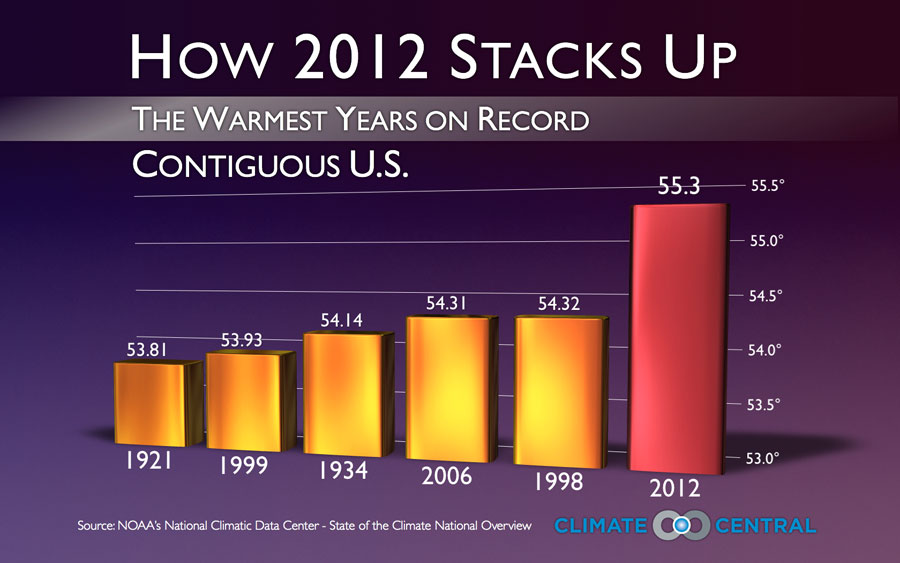
\includegraphics[scale=0.32]{./images/climate_bad}}
\end{figure}
\end{frame}
%%%%%%%%%%%%%%%%%%%%%%%%%%%%%%%%%%%%%%%%
\begin{frame}
\frametitle{Why is this one better?}
\framesubtitle{Source: \href{http://www.climatecentral.org/news/noaa-2012-was-warmest-and-second-most-extreme-year-on-record-15436}{\fbox{Climate Central}}}
	\begin{figure}
	\fbox{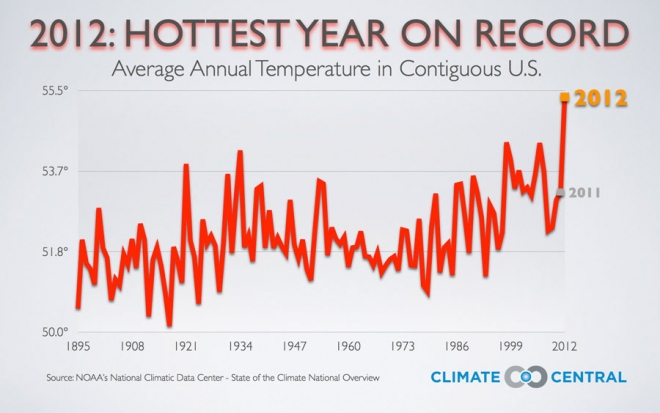
\includegraphics[scale=0.45]{./images/climate_good}}
\end{figure}
\end{frame}
%%%%%%%%%%%%%%%%%%%%%%%%%%%%%%%%%%%%%%%%
\begin{frame}
\begin{columns}
    \column{0.5\textwidth}
		\begin{figure}
	\fbox{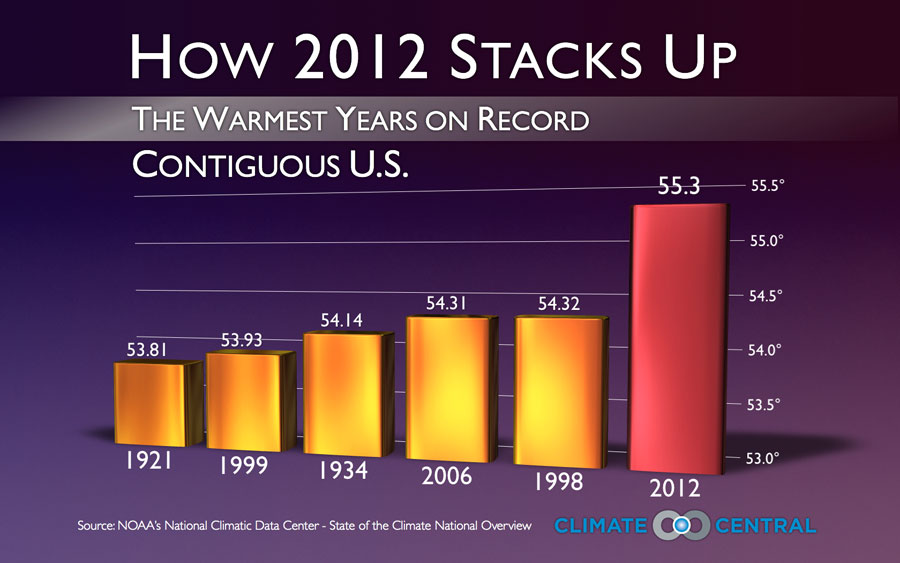
\includegraphics[scale=0.15]{./images/climate_bad}}
\end{figure}
	\footnotesize
	Bad Graph:
	\begin{itemize}
		\item Unnatural ordering of years
		\item 3-D effect (perspective) and y-axis exaggerate 2012
		\item Why \emph{six} warmest years?
		\item Lack of context: what about other 111 years?
		\item Gives no information on overall climate variability
	\end{itemize}
	
	\column{0.5\textwidth}
			\begin{figure}
	\fbox{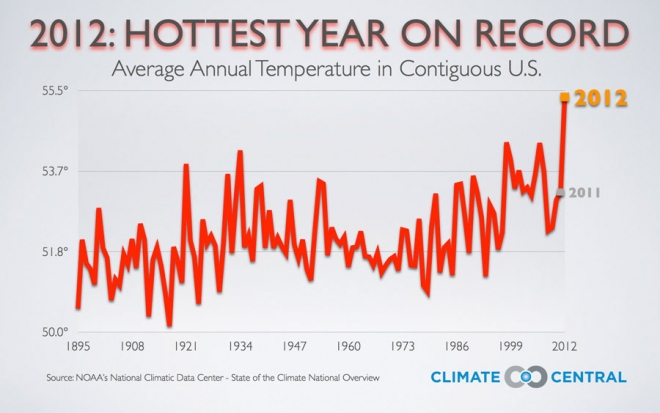
\includegraphics[scale=0.2]{./images/climate_good}}
		\small
\end{figure}
\footnotesize
Good Graph:
	\begin{itemize}
		\item Shows all years in order (context)
		\item Shows variability and trend
		\item y-axis chosen to comfortably fit all observations
		\item 2-D rather than 3-D
	\end{itemize}
	
	\vspace{5em}
\end{columns}

\end{frame}

%%%%%%%%%%%%%%%%%%%%%%%%%%%%%%%%%%%%%%%%
\begin{frame}

	\begin{block}{Why Graphics?}
	Humans naturally skilled at interpreting spatial information
	\end{block}


\begin{block}{Some Guidelines}
	\begin{itemize}
		\item Use \alert{distance} rather than area or perspective
		\item Avoid clutter (chartjunk)
		\item Use meaningful order where possible
		\item Make a \alert{visual argument}, not a work of art
	\end{itemize}
\end{block}

\end{frame}

%%%%%%%%%%%%%%%%%%%%%%%%%%%%%%%%%%%%%%%%
\begin{frame}
\singlespacing
\frametitle{Best Statistical Graphic \emph{Ever}}
\framesubtitle{Charles Joseph Minard, 1861 }
\begin{figure}
\framebox{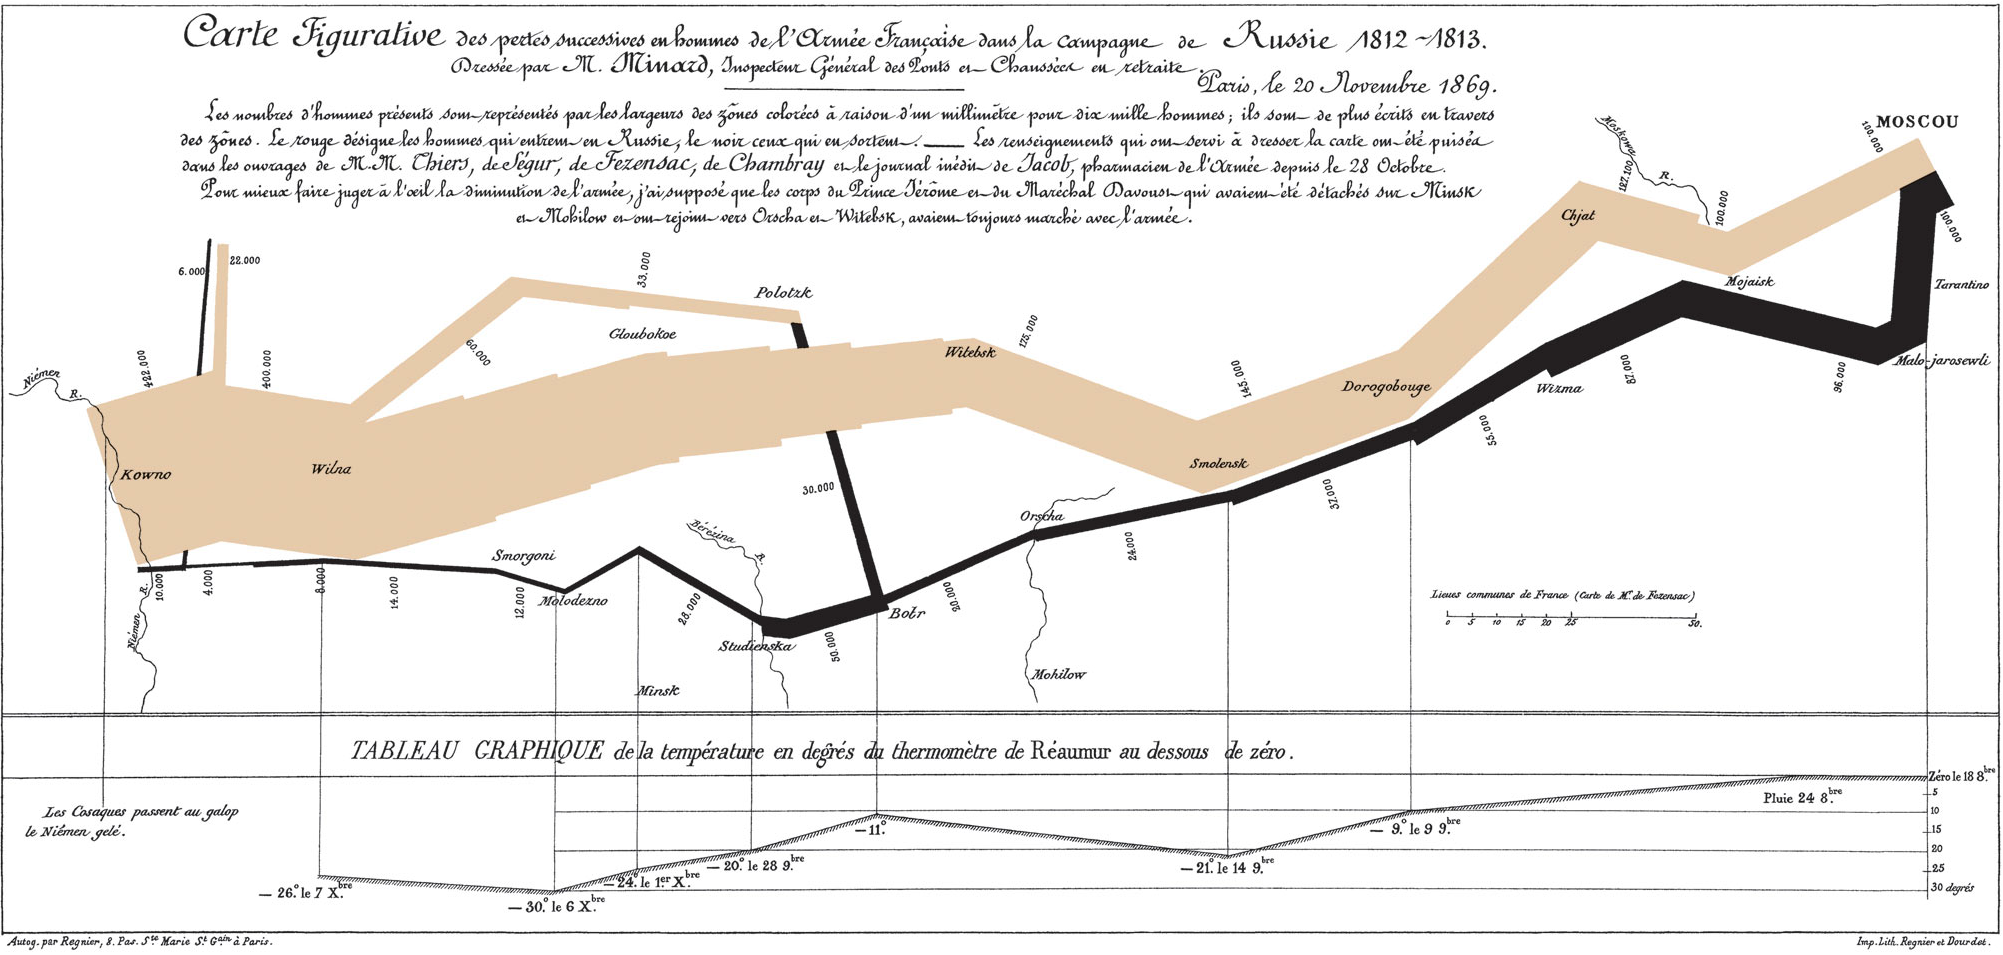
\includegraphics[scale = 0.20]{./images/Minard}}
\caption{Napoleon's disasterous Russian Campaign of 1812. Depicts six variables: temperature, location (two dimensions), direction, number of troops, and date.}
\end{figure}

\end{frame}


%%%%%%%%%%%%%%%%%%%%%%%%%%%%%%%%%%%%%%%%

%
%
%\begin{frame}
%\frametitle{Sideways is Often Better}
%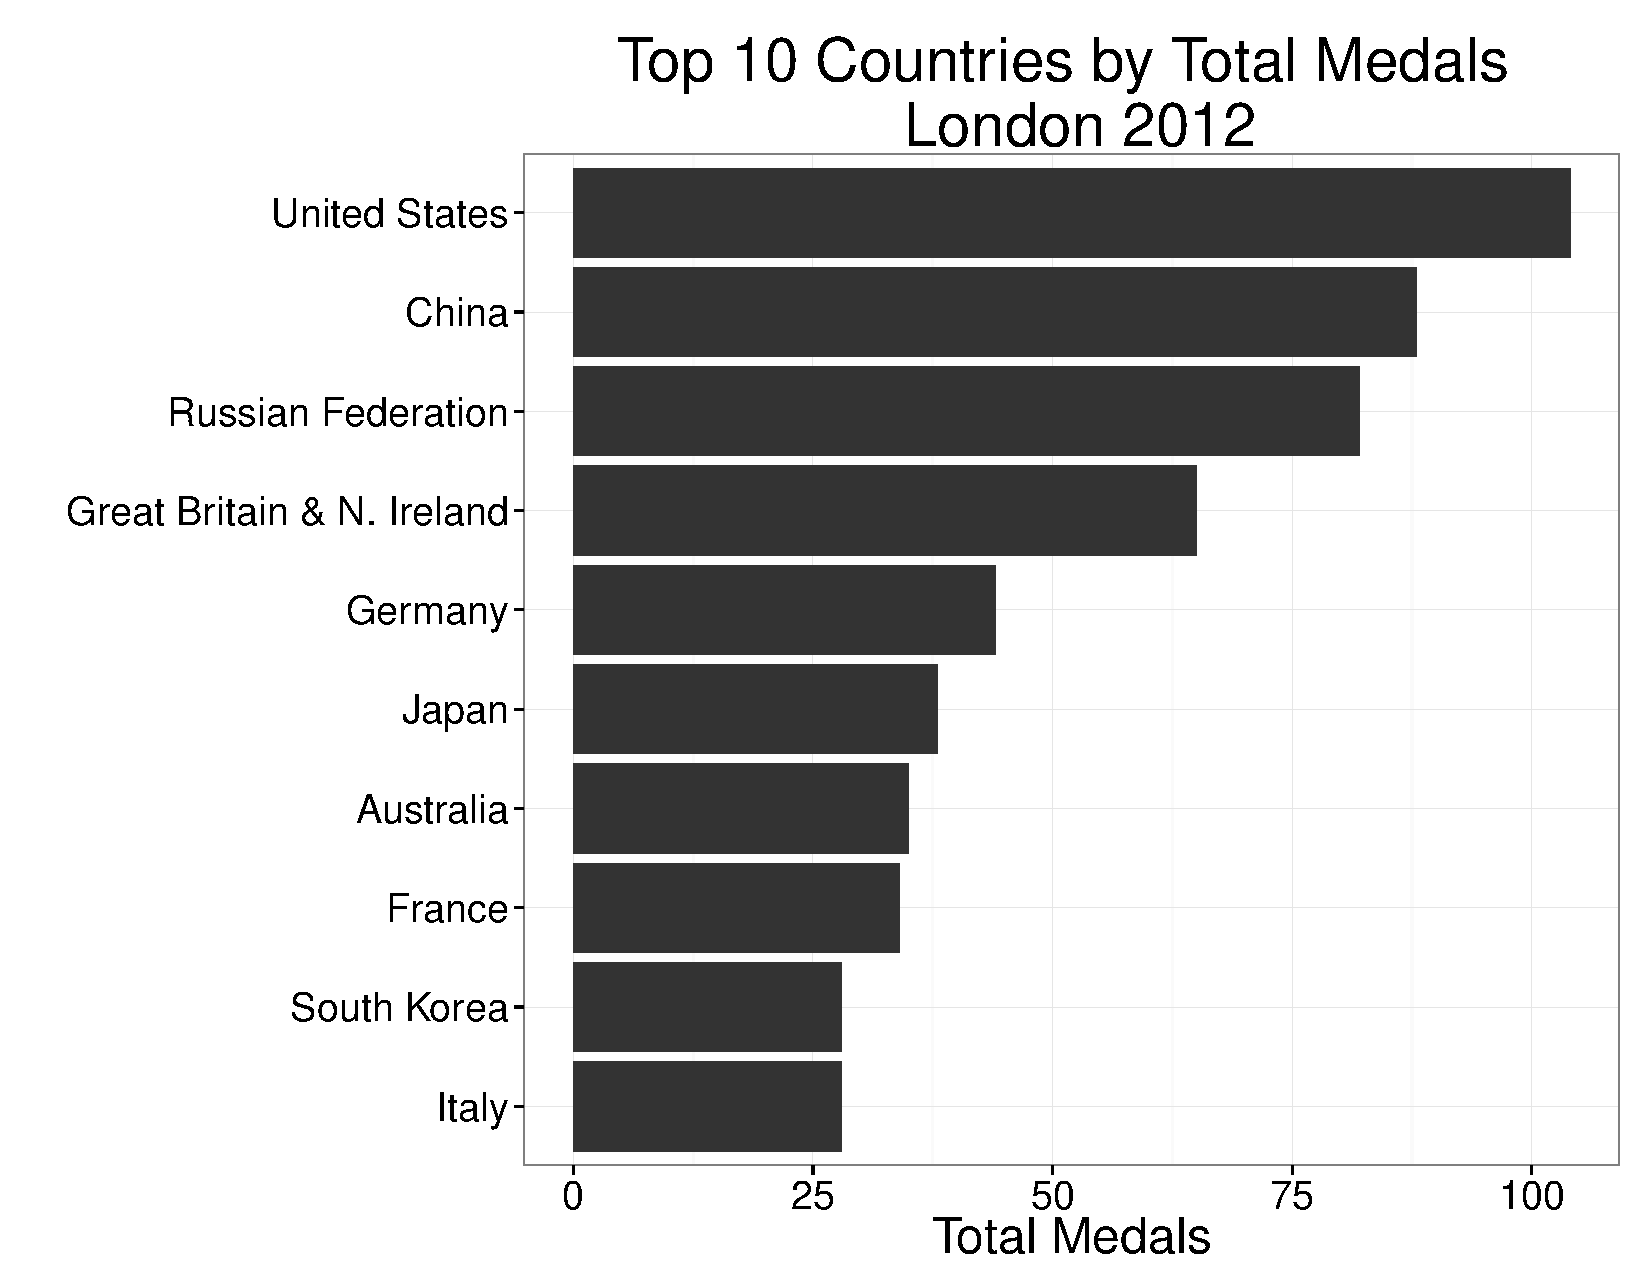
\includegraphics[scale = 0.38]{./images/medalcount_barchart}
%
%\end{frame}
%%%%%%%%%%%%%%%%%%%%%%%%%%%%%%%%%%%%%%%%%
%
%\begin{frame}
%\frametitle{Less Can be More -- The Dotchart}
%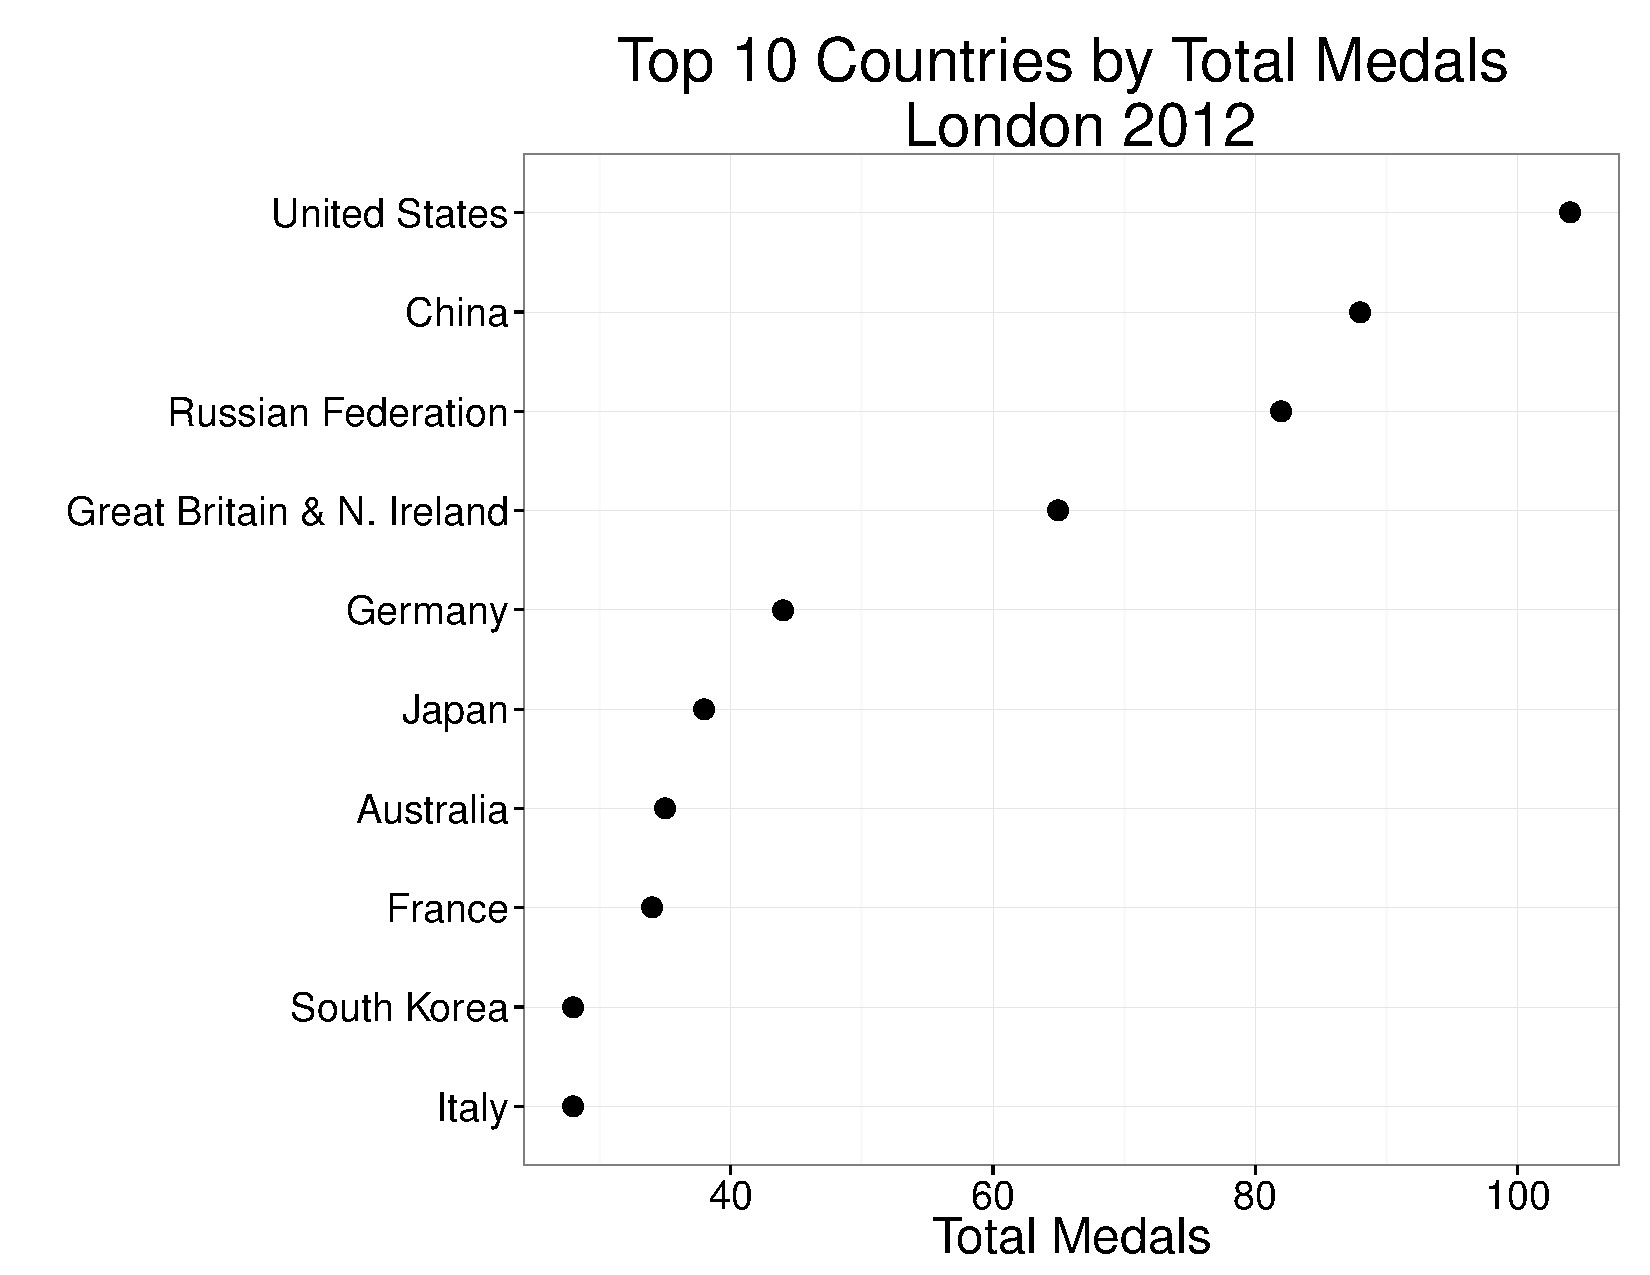
\includegraphics[scale = 0.35]{./images/medalcount_dotchart}
%
%
%\end{frame}
%%%%%%%%%%%%%%%%%%%%%%%%%%%%%%%%%%%%%%%%%
%
%\begin{frame}
%\frametitle{Friends Don't Let Friends Make Pie Charts}
%\centering
%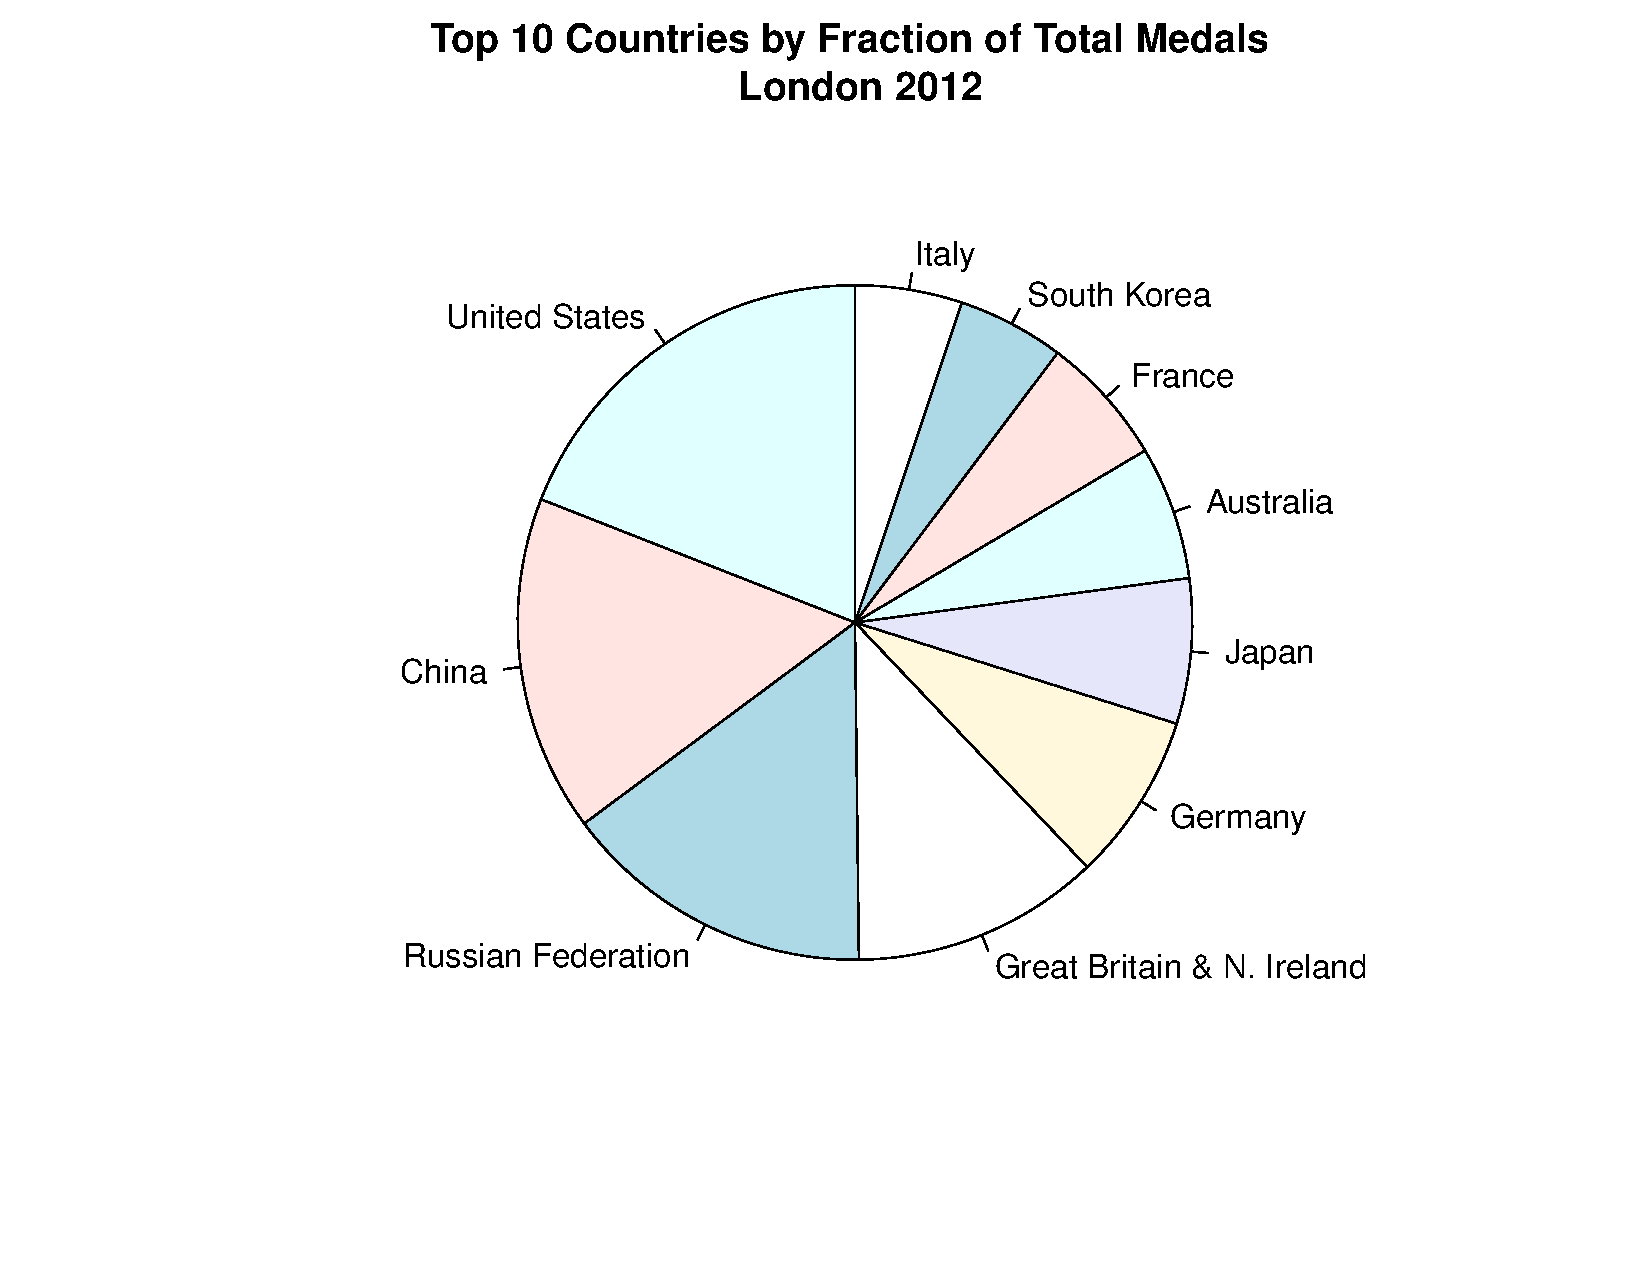
\includegraphics[scale = 0.4]{./images/London_pie}
%
%\end{frame}
%
%%%%%%%%%%%%%%%%%%%%%%%%%%%%%%%%%%%%%%%%%
%
%
%\begin{frame}
%\frametitle{Dotcharts (or Barcharts) Are Just Fine for Proportions!}
%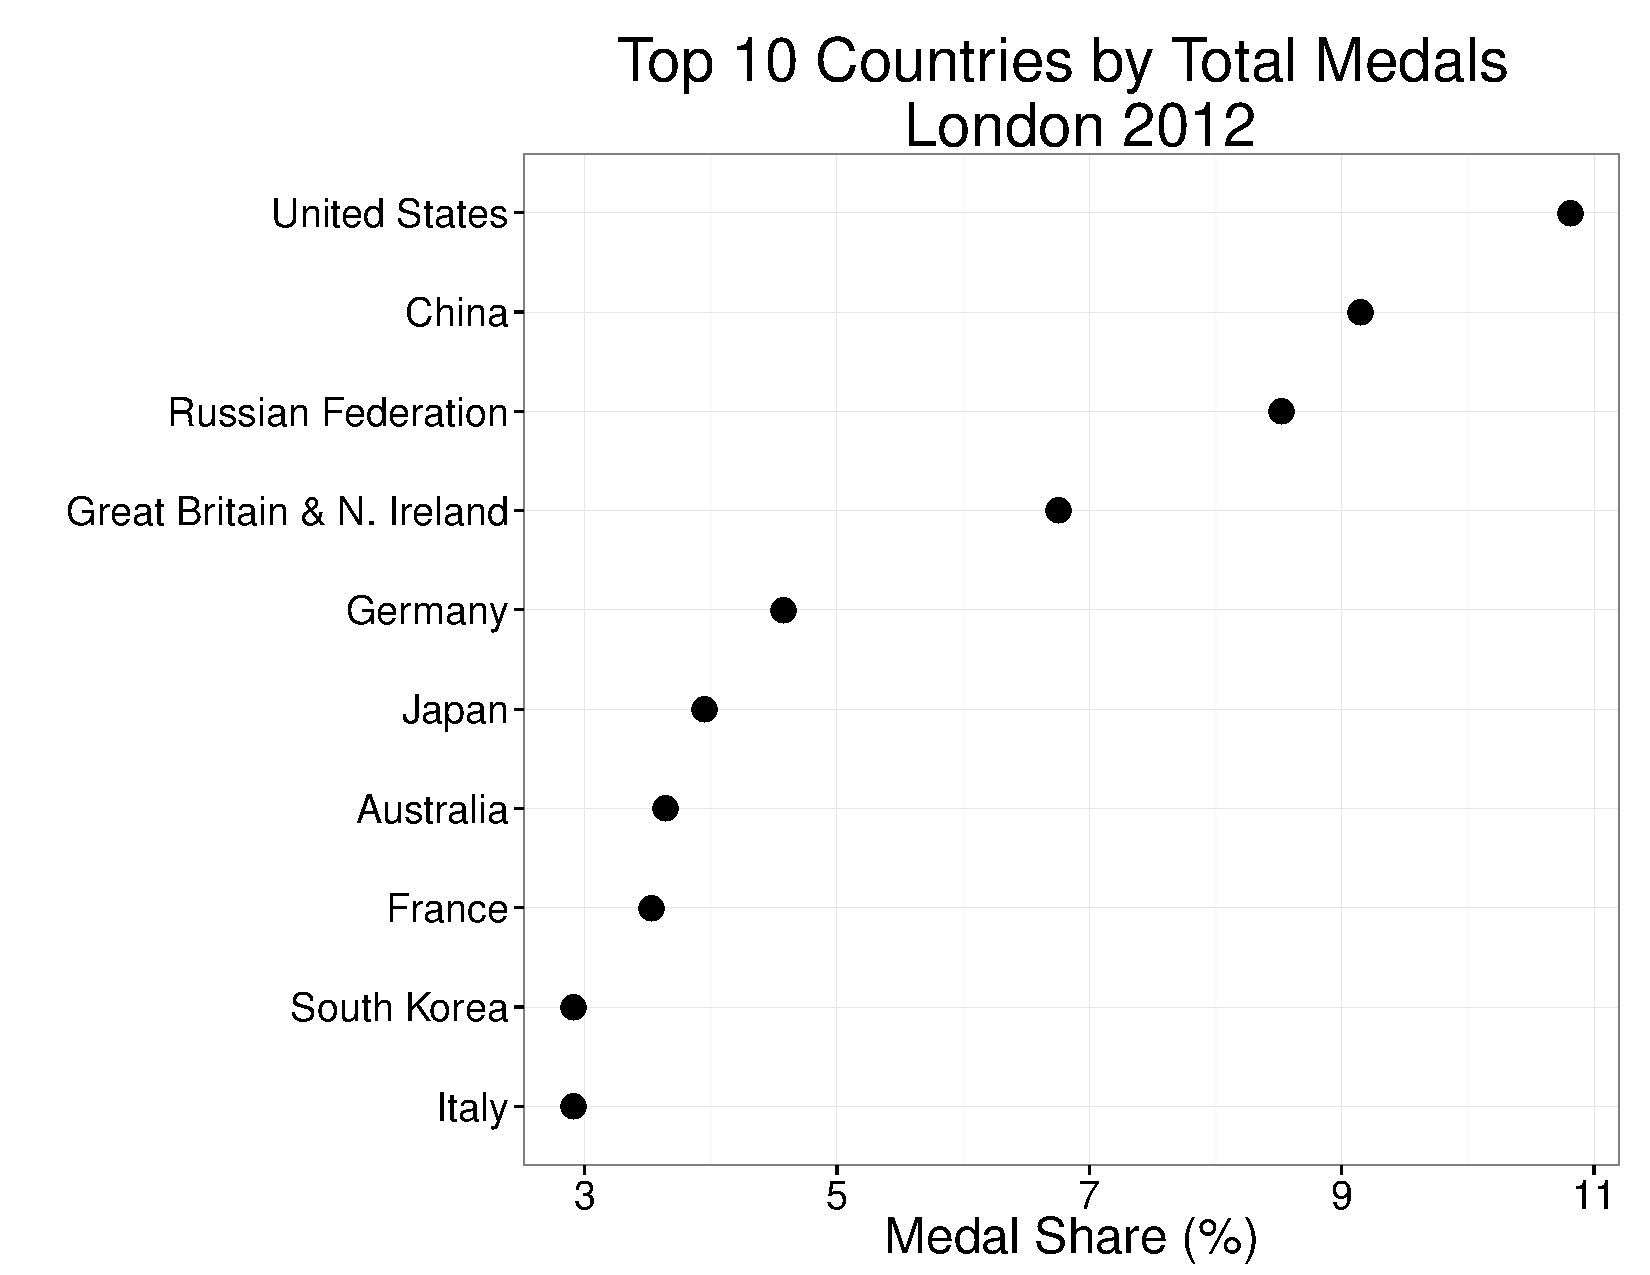
\includegraphics[scale = 0.35]{./images/medalshare_dotplot}
%
%\end{frame}
%
%%%%%%%%%%%%%%%%%%%%%%%%%%%%%%%%%%%%%%%%%
%
%\begin{frame}
%\frametitle{Stacked Barchart}
%\centering
%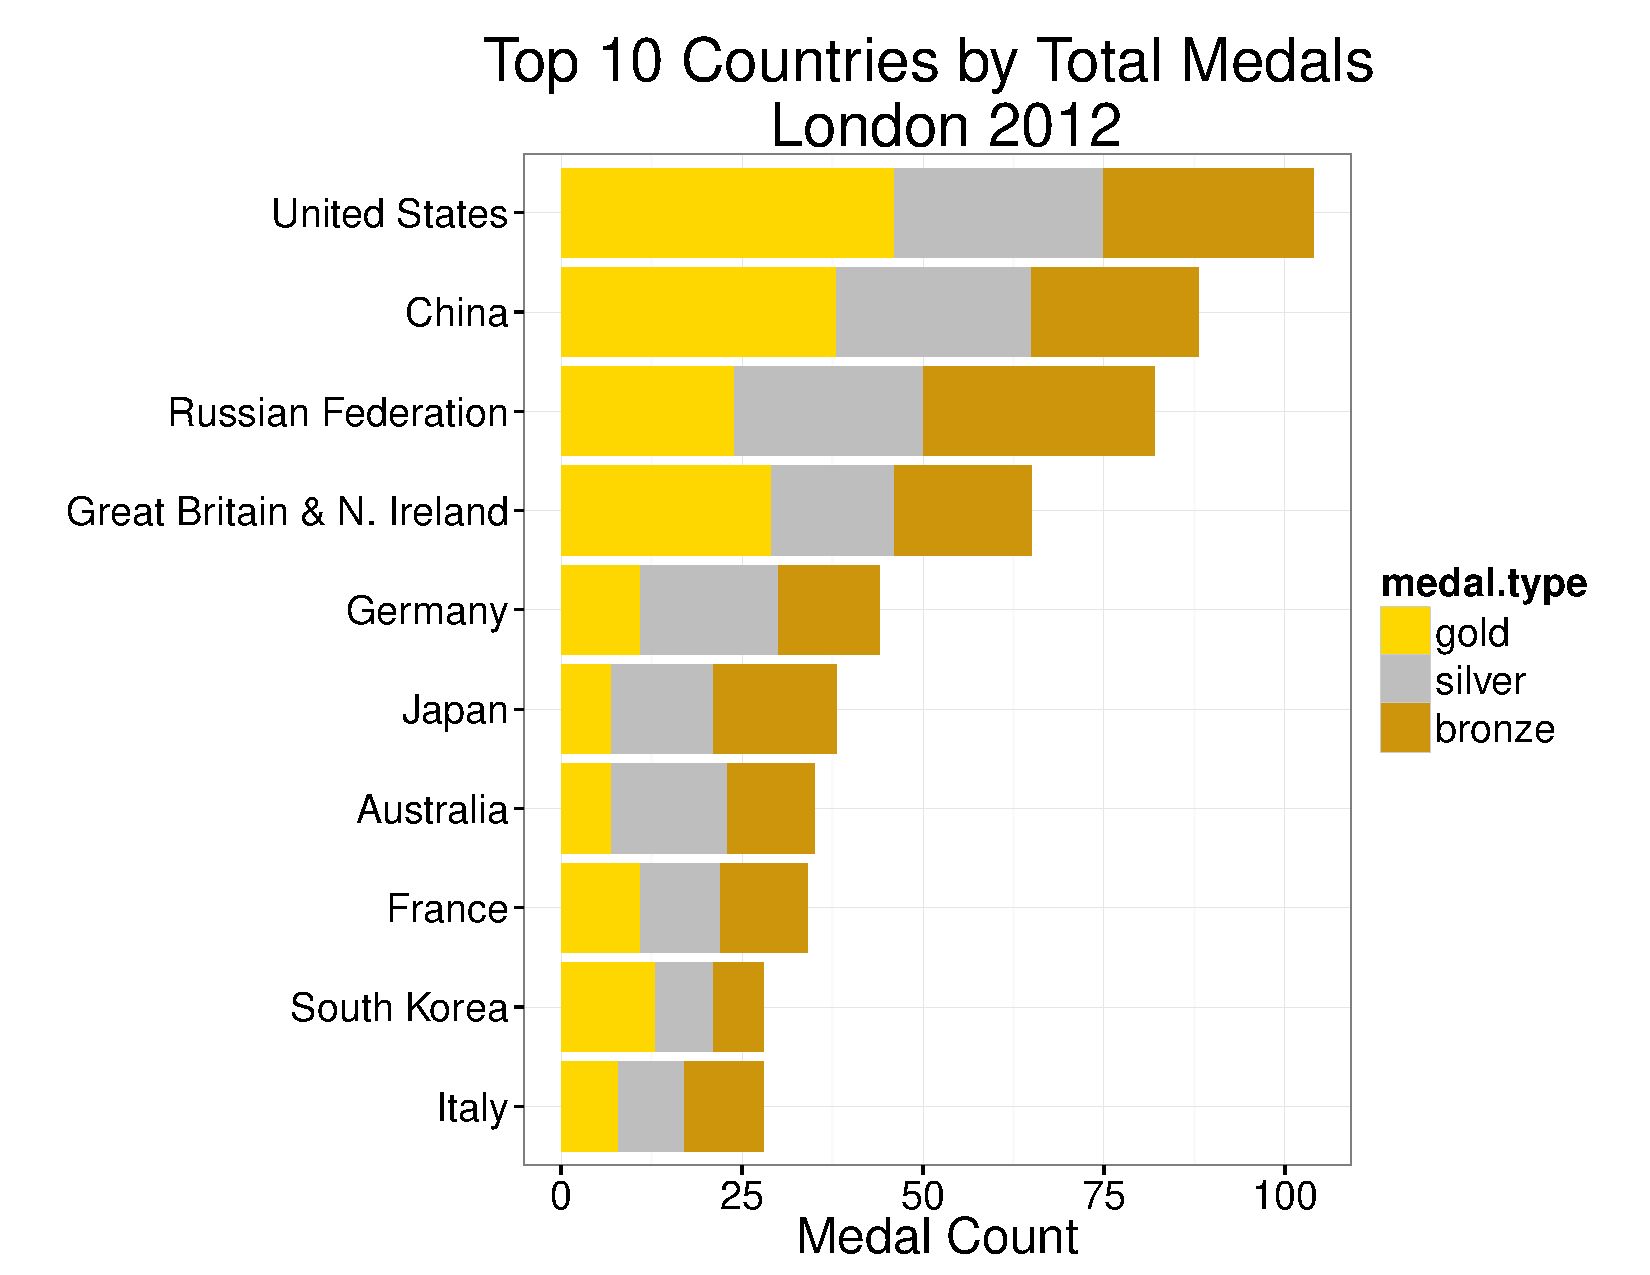
\includegraphics[scale = 0.35]{./images/medalcount_stacked_bar}
%
%\end{frame}
%
%%%%%%%%%%%%%%%%%%%%%%%%%%%%%%%%%%%%%%%%%
%
%\begin{frame}
%\frametitle{Multiple Dotcharts}
%\centering
%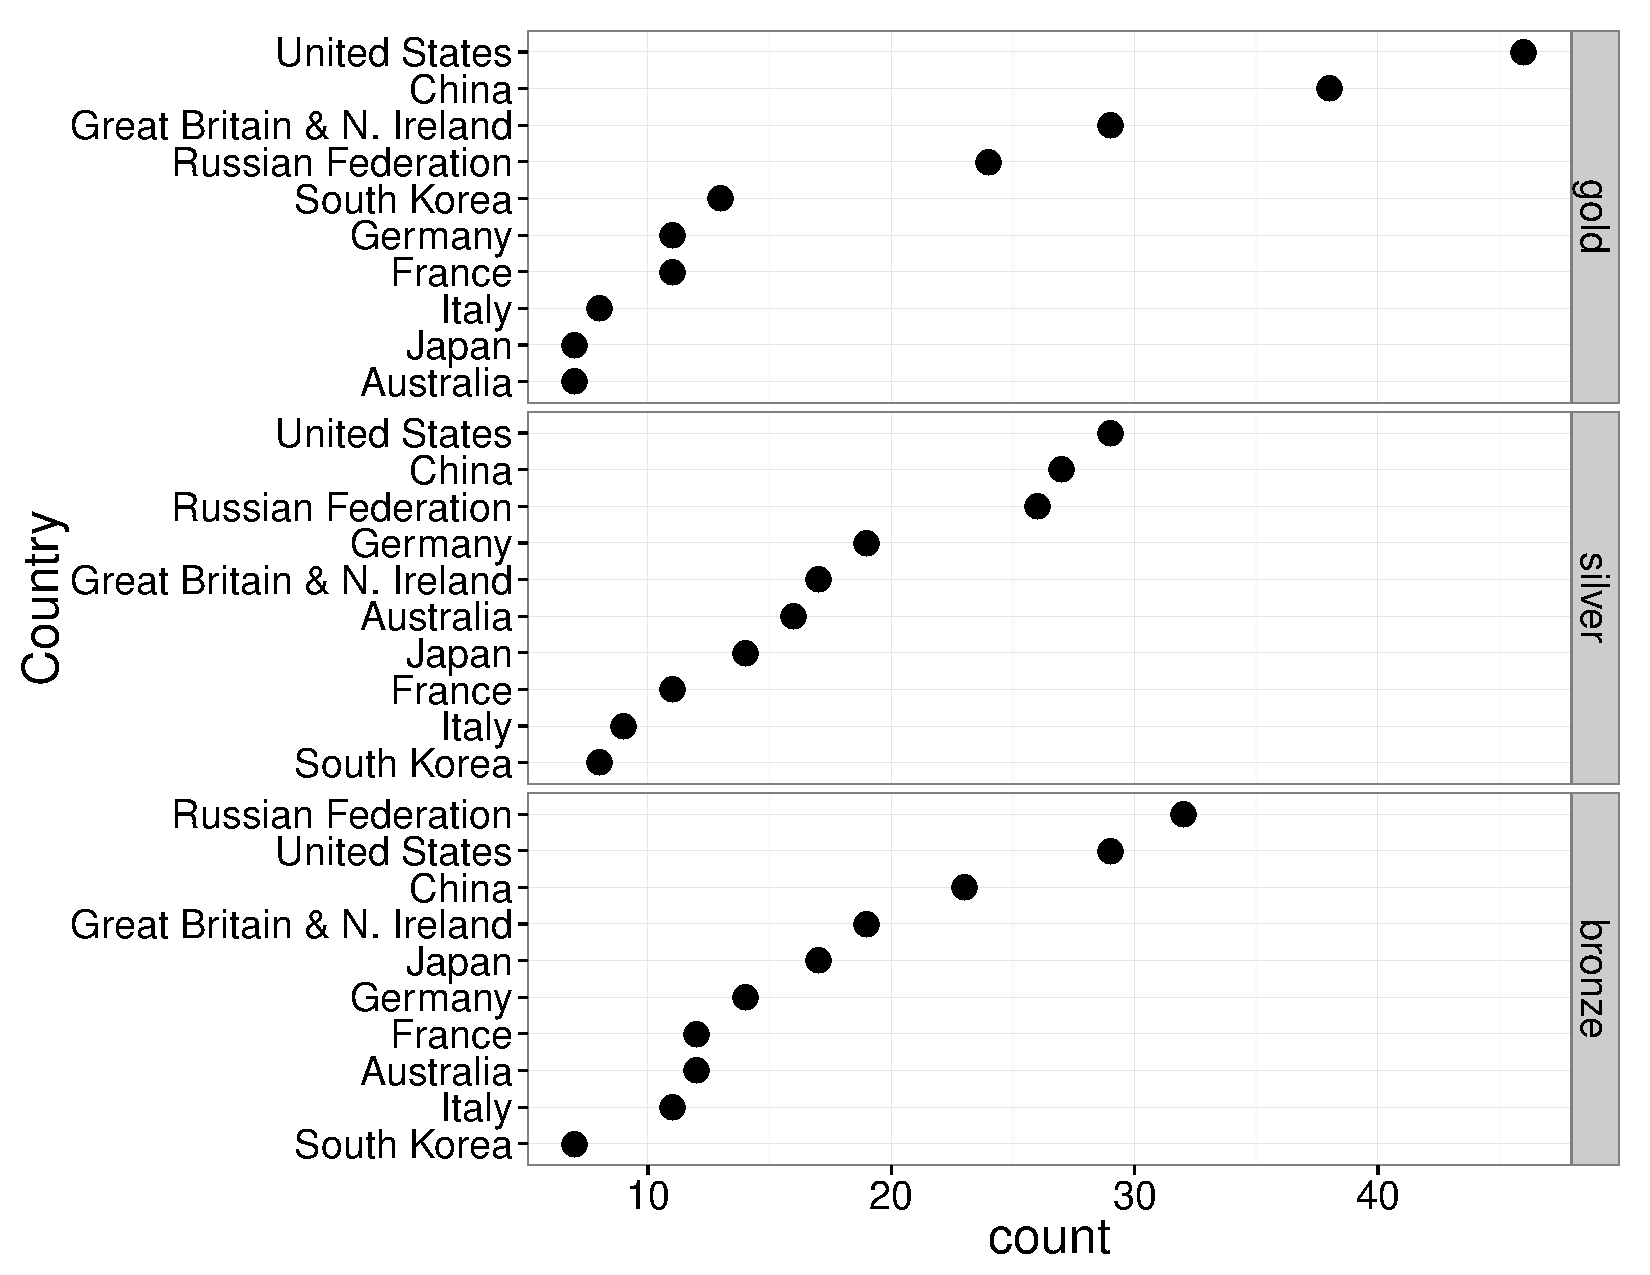
\includegraphics[scale = 0.35]{./images/medalcount_dotplot_stacked}
%
%\end{frame}


%%%%%%%%%%%%%%%%%%%%%%%%%%%%%%%%%%%%%%%%

%\begin{frame}
%\frametitle{\footnotesize Source: \href{http://www.aeaweb.org/articles.php?doi=10.1257/jep.26.1.165}{\fbox{Avery \& Turner (2012)}}}
%\begin{center}
%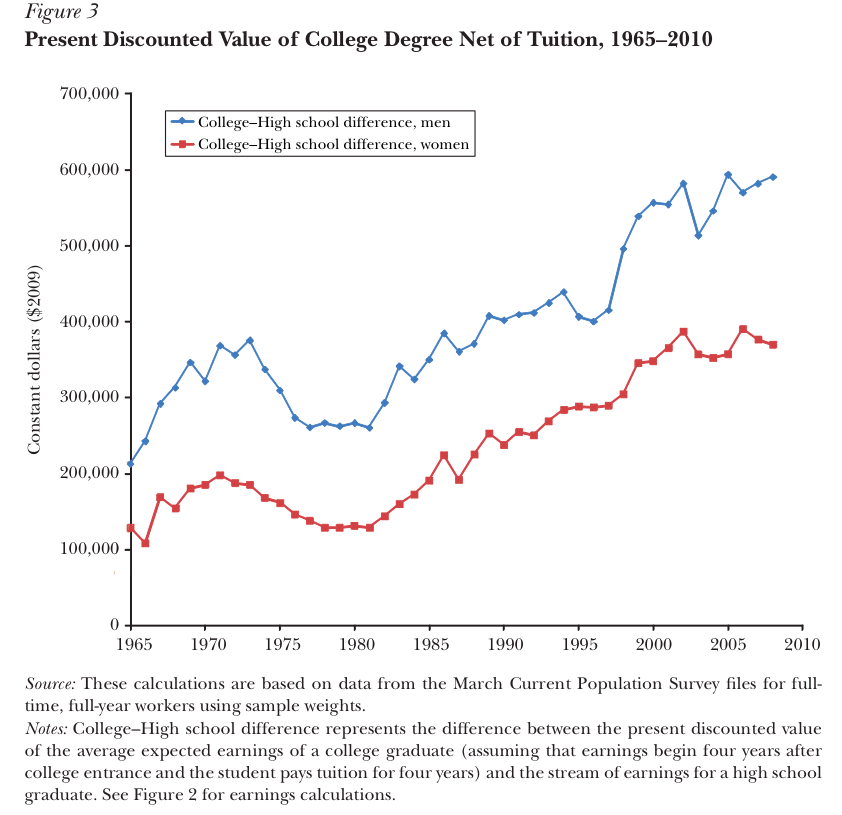
\includegraphics[scale = 0.28]{./images/tuition_line}
%\end{center}
%\end{frame}



%%%%%%%%%%%%%%%%%%%%%%%%%%%%%%%%%%%%%%%%



%\begin{frame}
%\begin{center}
%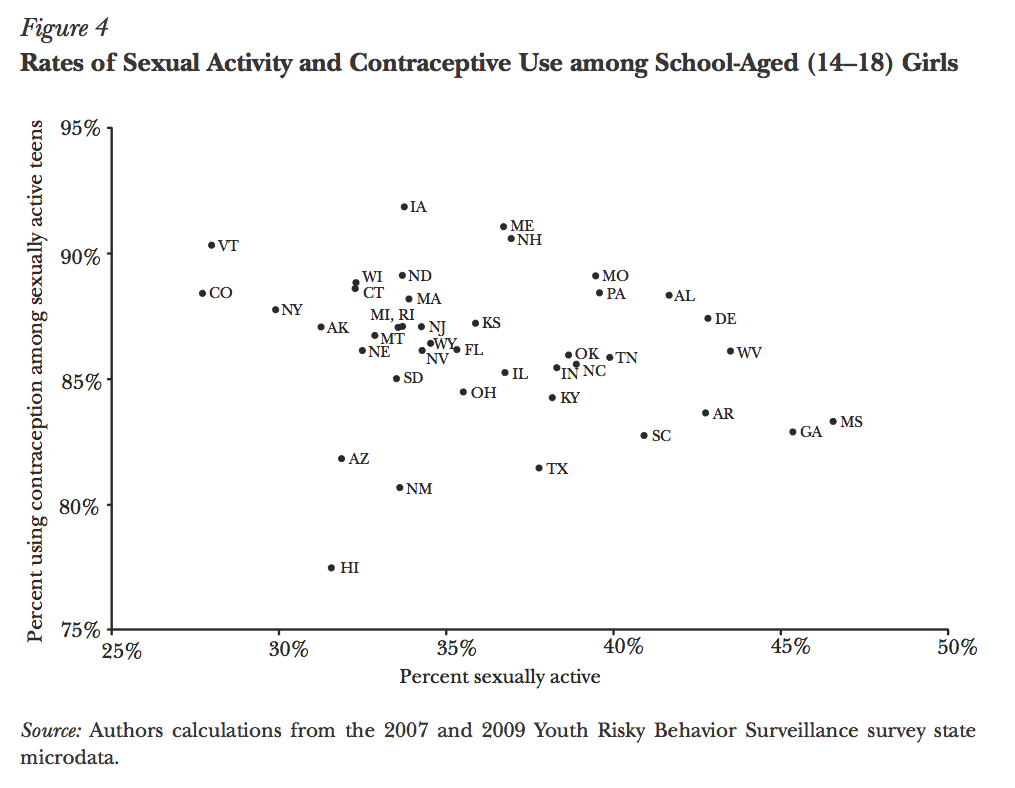
\includegraphics[scale = 0.3]{./images/scatter_teen_pregnancy}
%\end{center}
%\end{frame}

%%%%%%%%%%%%%%%%%%%%%%%%%%%%%%%%%%%%%%%%
\begin{frame}
\frametitle{Pairs Plot -- Handedness, Handspan and Height}
\begin{center}
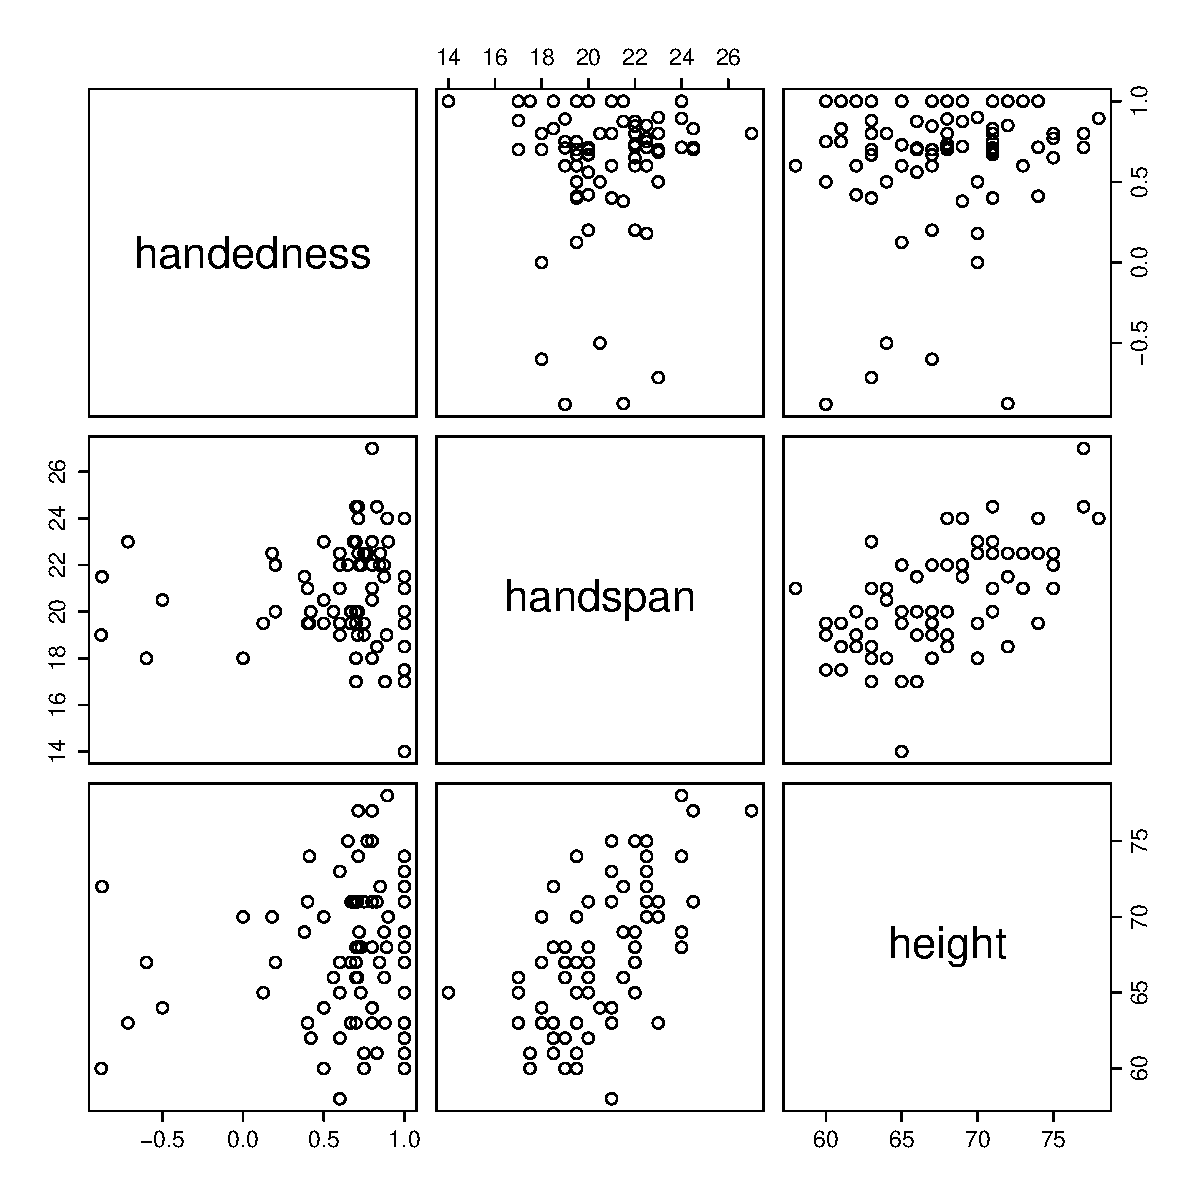
\includegraphics[scale = 0.38]{./images/pairs}
\end{center}
\end{frame}



%%%%%%%%%%%%%%%%%%%%%%%%%%%%%%%%%%%%%%%%



\begin{frame}
\frametitle{Bubblechart -- 2005 Crime Rates by State}
\framesubtitle{Source: \href{http://flowingdata.com}{\fbox{Flowing Data}}}
\centering
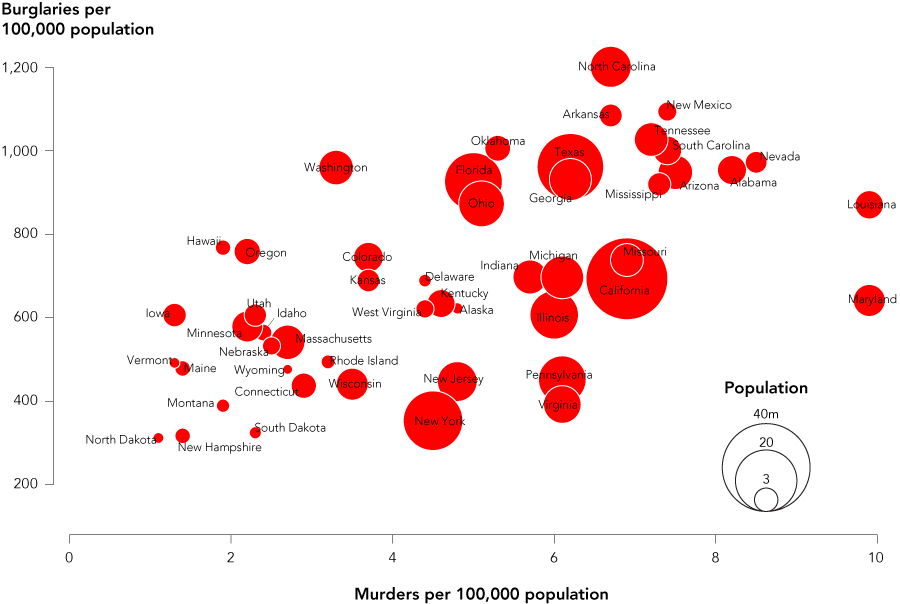
\includegraphics[scale = 0.30]{./images/crime_bubble2}

\end{frame}

%%%%%%%%%%%%%%%%%%%%%%%%%%%%%%%%%%%%%%%%

%\begin{frame}
%\begin{figure}
%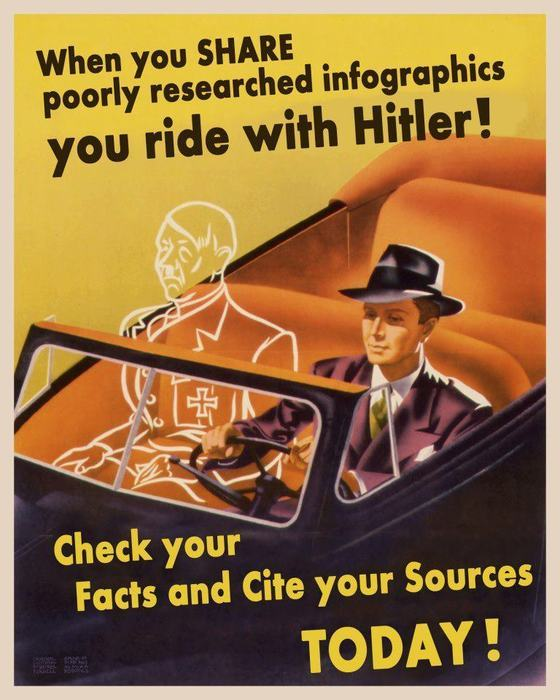
\includegraphics[scale = 0.35]{./images/infographics_hitler}
%\end{figure}

%\end{frame}

%%%%%%%%%%%%%%%%%%%%%%%%%%%%%%%%%%%%%%%%

\
